\documentclass[1p]{elsarticle_modified}
%\bibliographystyle{elsarticle-num}

%\usepackage[colorlinks]{hyperref}
%\usepackage{abbrmath_seonhwa} %\Abb, \Ascr, \Acal ,\Abf, \Afrak
\usepackage{amsfonts}
\usepackage{amssymb}
\usepackage{amsmath}
\usepackage{amsthm}
\usepackage{scalefnt}
\usepackage{amsbsy}
\usepackage{kotex}
\usepackage{caption}
\usepackage{subfig}
\usepackage{color}
\usepackage{graphicx}
\usepackage{xcolor} %% white, black, red, green, blue, cyan, magenta, yellow
\usepackage{float}
\usepackage{setspace}
\usepackage{hyperref}

\usepackage{tikz}
\usetikzlibrary{arrows}

\usepackage{multirow}
\usepackage{array} % fixed length table
\usepackage{hhline}

%%%%%%%%%%%%%%%%%%%%%
\makeatletter
\renewcommand*\env@matrix[1][\arraystretch]{%
	\edef\arraystretch{#1}%
	\hskip -\arraycolsep
	\let\@ifnextchar\new@ifnextchar
	\array{*\c@MaxMatrixCols c}}
\makeatother %https://tex.stackexchange.com/questions/14071/how-can-i-increase-the-line-spacing-in-a-matrix
%%%%%%%%%%%%%%%

\usepackage[normalem]{ulem}

\newcommand{\msout}[1]{\ifmmode\text{\sout{\ensuremath{#1}}}\else\sout{#1}\fi}
%SOURCE: \msout is \stkout macro in https://tex.stackexchange.com/questions/20609/strikeout-in-math-mode

\newcommand{\cancel}[1]{
	\ifmmode
	{\color{red}\msout{#1}}
	\else
	{\color{red}\sout{#1}}
	\fi
}

\newcommand{\add}[1]{
	{\color{blue}\uwave{#1}}
}

\newcommand{\replace}[2]{
	\ifmmode
	{\color{red}\msout{#1}}{\color{blue}\uwave{#2}}
	\else
	{\color{red}\sout{#1}}{\color{blue}\uwave{#2}}
	\fi
}

\newcommand{\Sol}{\mathcal{S}} %segment
\newcommand{\D}{D} %diagram
\newcommand{\A}{\mathcal{A}} %arc


%%%%%%%%%%%%%%%%%%%%%%%%%%%%%5 test

\def\sl{\operatorname{\textup{SL}}(2,\Cbb)}
\def\psl{\operatorname{\textup{PSL}}(2,\Cbb)}
\def\quan{\mkern 1mu \triangleright \mkern 1mu}

\theoremstyle{definition}
\newtheorem{thm}{Theorem}[section]
\newtheorem{prop}[thm]{Proposition}
\newtheorem{lem}[thm]{Lemma}
\newtheorem{ques}[thm]{Question}
\newtheorem{cor}[thm]{Corollary}
\newtheorem{defn}[thm]{Definition}
\newtheorem{exam}[thm]{Example}
\newtheorem{rmk}[thm]{Remark}
\newtheorem{alg}[thm]{Algorithm}

\newcommand{\I}{\sqrt{-1}}
\begin{document}

%\begin{frontmatter}
%
%\title{Boundary parabolic representations of knots up to 8 crossings}
%
%%% Group authors per affiliation:
%\author{Yunhi Cho} 
%\address{Department of Mathematics, University of Seoul, Seoul, Korea}
%\ead{yhcho@uos.ac.kr}
%
%
%\author{Seonhwa Kim} %\fnref{s_kim}}
%\address{Center for Geometry and Physics, Institute for Basic Science, Pohang, 37673, Korea}
%\ead{ryeona17@ibs.re.kr}
%
%\author{Hyuk Kim}
%\address{Department of Mathematical Sciences, Seoul National University, Seoul 08826, Korea}
%\ead{hyukkim@snu.ac.kr}
%
%\author{Seokbeom Yoon}
%\address{Department of Mathematical Sciences, Seoul National University, Seoul, 08826,  Korea}
%\ead{sbyoon15@snu.ac.kr}
%
%\begin{abstract}
%We find all boundary parabolic representation of knots up to 8 crossings.
%
%\end{abstract}
%\begin{keyword}
%    \MSC[2010] 57M25 
%\end{keyword}
%
%\end{frontmatter}

%\linenumbers
%\tableofcontents
%
\newcommand\colored[1]{\textcolor{white}{\rule[-0.35ex]{0.8em}{1.4ex}}\kern-0.8em\color{red} #1}%
%\newcommand\colored[1]{\textcolor{white}{ #1}\kern-2.17ex	\textcolor{white}{ #1}\kern-1.81ex	\textcolor{white}{ #1}\kern-2.15ex\color{red}#1	}

{\Large $\underline{12a_{0313}~(K12a_{0313})}$}

\setlength{\tabcolsep}{10pt}
\renewcommand{\arraystretch}{1.6}
\vspace{1cm}\begin{tabular}{m{100pt}>{\centering\arraybackslash}m{274pt}}
\multirow{5}{120pt}{
	\centering
	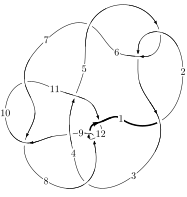
\includegraphics[width=112pt]{../../../GIT/diagram.site/Diagrams/png/1114_12a_0313.png}\\
\ \ \ A knot diagram\footnotemark}&
\allowdisplaybreaks
\textbf{Linearized knot diagam} \\
\cline{2-2}
 &
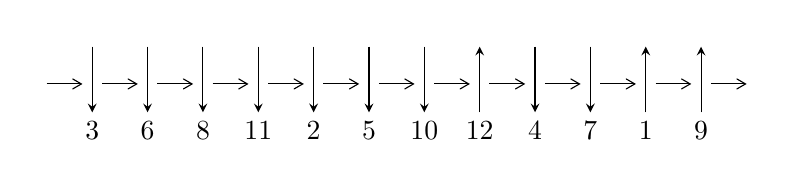
\begin{tikzpicture}[x=20pt, y=17pt]
	% nodes
	\node (C0) at (0, 0) {};
	\node (C1) at (1, 0) {};
	\node (C1U) at (1, +1) {};
	\node (C1D) at (1, -1) {3};

	\node (C2) at (2, 0) {};
	\node (C2U) at (2, +1) {};
	\node (C2D) at (2, -1) {6};

	\node (C3) at (3, 0) {};
	\node (C3U) at (3, +1) {};
	\node (C3D) at (3, -1) {8};

	\node (C4) at (4, 0) {};
	\node (C4U) at (4, +1) {};
	\node (C4D) at (4, -1) {11};

	\node (C5) at (5, 0) {};
	\node (C5U) at (5, +1) {};
	\node (C5D) at (5, -1) {2};

	\node (C6) at (6, 0) {};
	\node (C6U) at (6, +1) {};
	\node (C6D) at (6, -1) {5};

	\node (C7) at (7, 0) {};
	\node (C7U) at (7, +1) {};
	\node (C7D) at (7, -1) {10};

	\node (C8) at (8, 0) {};
	\node (C8U) at (8, +1) {};
	\node (C8D) at (8, -1) {12};

	\node (C9) at (9, 0) {};
	\node (C9U) at (9, +1) {};
	\node (C9D) at (9, -1) {4};

	\node (C10) at (10, 0) {};
	\node (C10U) at (10, +1) {};
	\node (C10D) at (10, -1) {7};

	\node (C11) at (11, 0) {};
	\node (C11U) at (11, +1) {};
	\node (C11D) at (11, -1) {1};

	\node (C12) at (12, 0) {};
	\node (C12U) at (12, +1) {};
	\node (C12D) at (12, -1) {9};
	\node (C13) at (13, 0) {};

	% arrows
	\draw[->,>={angle 60}]
	(C0) edge (C1) (C1) edge (C2) (C2) edge (C3) (C3) edge (C4) (C4) edge (C5) (C5) edge (C6) (C6) edge (C7) (C7) edge (C8) (C8) edge (C9) (C9) edge (C10) (C10) edge (C11) (C11) edge (C12) (C12) edge (C13) ;	\draw[->,>=stealth]
	(C1U) edge (C1D) (C2U) edge (C2D) (C3U) edge (C3D) (C4U) edge (C4D) (C5U) edge (C5D) (C6U) edge (C6D) (C7U) edge (C7D) (C8D) edge (C8U) (C9U) edge (C9D) (C10U) edge (C10D) (C11D) edge (C11U) (C12D) edge (C12U) ;
	\end{tikzpicture} \\
\hhline{~~} \\& 
\textbf{Solving Sequence} \\ \cline{2-2} 
 &
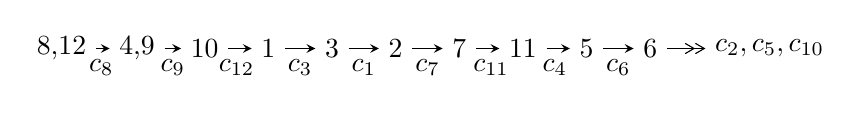
\begin{tikzpicture}[x=23pt, y=7pt]
	% node
	\node (A0) at (-1/8, 0) {8,12};
	\node (A1) at (17/16, 0) {4,9};
	\node (A2) at (17/8, 0) {10};
	\node (A3) at (25/8, 0) {1};
	\node (A4) at (33/8, 0) {3};
	\node (A5) at (41/8, 0) {2};
	\node (A6) at (49/8, 0) {7};
	\node (A7) at (57/8, 0) {11};
	\node (A8) at (65/8, 0) {5};
	\node (A9) at (73/8, 0) {6};
	\node (C1) at (1/2, -1) {$c_{8}$};
	\node (C2) at (13/8, -1) {$c_{9}$};
	\node (C3) at (21/8, -1) {$c_{12}$};
	\node (C4) at (29/8, -1) {$c_{3}$};
	\node (C5) at (37/8, -1) {$c_{1}$};
	\node (C6) at (45/8, -1) {$c_{7}$};
	\node (C7) at (53/8, -1) {$c_{11}$};
	\node (C8) at (61/8, -1) {$c_{4}$};
	\node (C9) at (69/8, -1) {$c_{6}$};
	\node (A10) at (11, 0) {$c_{2},c_{5},c_{10}$};

	% edge
	\draw[->,>=stealth]	
	(A0) edge (A1) (A1) edge (A2) (A2) edge (A3) (A3) edge (A4) (A4) edge (A5) (A5) edge (A6) (A6) edge (A7) (A7) edge (A8) (A8) edge (A9) ;
	\draw[->>,>={angle 60}]	
	(A9) edge (A10);
\end{tikzpicture} \\ 

\end{tabular} \\

\footnotetext{
The image of knot diagram is generated by the software ``\textbf{Draw programme}" developed by Andrew Bartholomew(\url{http://www.layer8.co.uk/maths/draw/index.htm\#Running-draw}), where we modified some parts for our purpose(\url{https://github.com/CATsTAILs/LinksPainter}).
}\phantom \\ \newline 
\centering \textbf{Ideals for irreducible components\footnotemark of $X_{\text{par}}$} 
 
\begin{align*}
I^u_{1}&=\langle 
-1.70812\times10^{157} u^{106}-3.03141\times10^{158} u^{105}+\cdots+2.56694\times10^{158} b+6.21022\times10^{158},\\
\phantom{I^u_{1}}&\phantom{= \langle  }1.09767\times10^{160} u^{106}+6.85071\times10^{160} u^{105}+\cdots+7.18742\times10^{159} a-1.03525\times10^{160},\;u^{107}+7 u^{106}+\cdots-7 u-2\rangle \\
I^u_{2}&=\langle 
- u^3+b+u+1,\;u^3+u^2+a+u-1,\;u^4- u^2+1\rangle \\
\\
\end{align*}
\raggedright * 2 irreducible components of $\dim_{\mathbb{C}}=0$, with total 111 representations.\\
\footnotetext{All coefficients of polynomials are rational numbers. But the coefficients are sometimes approximated in decimal forms when there is not enough margin.}
\newpage
\renewcommand{\arraystretch}{1}
\centering \section*{I. $I^u_{1}= \langle -1.71\times10^{157} u^{106}-3.03\times10^{158} u^{105}+\cdots+2.57\times10^{158} b+6.21\times10^{158},\;1.10\times10^{160} u^{106}+6.85\times10^{160} u^{105}+\cdots+7.19\times10^{159} a-1.04\times10^{160},\;u^{107}+7 u^{106}+\cdots-7 u-2 \rangle$}
\flushleft \textbf{(i) Arc colorings}\\
\begin{tabular}{m{7pt} m{180pt} m{7pt} m{180pt} }
\flushright $a_{8}=$&$\begin{pmatrix}1\\0\end{pmatrix}$ \\
\flushright $a_{12}=$&$\begin{pmatrix}0\\u\end{pmatrix}$ \\
\flushright $a_{4}=$&$\begin{pmatrix}-1.52721 u^{106}-9.53153 u^{105}+\cdots+11.6434 u+1.44036\\0.0665430 u^{106}+1.18095 u^{105}+\cdots-2.78415 u-2.41931\end{pmatrix}$ \\
\flushright $a_{9}=$&$\begin{pmatrix}1\\- u^2\end{pmatrix}$ \\
\flushright $a_{10}=$&$\begin{pmatrix}-0.906926 u^{106}-6.15088 u^{105}+\cdots+12.2394 u+4.67446\\-0.0941909 u^{106}-0.564758 u^{105}+\cdots+1.37335 u+0.115362\end{pmatrix}$ \\
\flushright $a_{1}=$&$\begin{pmatrix}u\\- u^3+u\end{pmatrix}$ \\
\flushright $a_{3}=$&$\begin{pmatrix}-1.46067 u^{106}-8.35058 u^{105}+\cdots+8.85926 u-0.978951\\0.0665430 u^{106}+1.18095 u^{105}+\cdots-2.78415 u-2.41931\end{pmatrix}$ \\
\flushright $a_{2}=$&$\begin{pmatrix}-1.38743 u^{106}-8.09403 u^{105}+\cdots+0.613109 u+0.639209\\-0.318537 u^{106}-1.68135 u^{105}+\cdots+1.60195 u+0.444072\end{pmatrix}$ \\
\flushright $a_{7}=$&$\begin{pmatrix}-1.07925 u^{106}-6.86061 u^{105}+\cdots-2.88963 u+1.87350\\-0.628187 u^{106}-3.75798 u^{105}+\cdots+2.64801 u+1.32955\end{pmatrix}$ \\
\flushright $a_{11}=$&$\begin{pmatrix}- u^3\\u^5- u^3+u\end{pmatrix}$ \\
\flushright $a_{5}=$&$\begin{pmatrix}-1.07654 u^{106}-6.14521 u^{105}+\cdots+8.78359 u-0.113308\\-0.188990 u^{106}-0.943983 u^{105}+\cdots+0.658999 u-0.957025\end{pmatrix}$ \\
\flushright $a_{6}=$&$\begin{pmatrix}0.277869 u^{106}+1.24570 u^{105}+\cdots-1.71526 u+1.88041\\-0.108162 u^{106}-0.980032 u^{105}+\cdots+1.06338 u+0.961280\end{pmatrix}$\\&\end{tabular}
\flushleft \textbf{(ii) Obstruction class $= -1$}\\~\\
\flushleft \textbf{(iii) Cusp Shapes $= 1.55581 u^{106}+12.7480 u^{105}+\cdots-20.5992 u-13.0896$}\\~\\
\newpage\renewcommand{\arraystretch}{1}
\flushleft \textbf{(iv) u-Polynomials at the component}\newline \\
\begin{tabular}{m{50pt}|m{274pt}}
Crossings & \hspace{64pt}u-Polynomials at each crossing \\
\hline $$\begin{aligned}c_{1},c_{6}\end{aligned}$$&$\begin{aligned}
&u^{107}+33 u^{106}+\cdots+16 u+1
\end{aligned}$\\
\hline $$\begin{aligned}c_{2},c_{5}\end{aligned}$$&$\begin{aligned}
&u^{107}+5 u^{106}+\cdots+6 u+1
\end{aligned}$\\
\hline $$\begin{aligned}c_{3}\end{aligned}$$&$\begin{aligned}
&u^{107}-9 u^{106}+\cdots+51550 u+30431
\end{aligned}$\\
\hline $$\begin{aligned}c_{4}\end{aligned}$$&$\begin{aligned}
&u^{107}-29 u^{106}+\cdots-71644122 u+19604249
\end{aligned}$\\
\hline $$\begin{aligned}c_{7},c_{10}\end{aligned}$$&$\begin{aligned}
&u^{107}-7 u^{106}+\cdots-32 u+1
\end{aligned}$\\
\hline $$\begin{aligned}c_{8},c_{12}\end{aligned}$$&$\begin{aligned}
&u^{107}-7 u^{106}+\cdots-7 u+2
\end{aligned}$\\
\hline $$\begin{aligned}c_{9}\end{aligned}$$&$\begin{aligned}
&u^{107}- u^{106}+\cdots-18 u+1
\end{aligned}$\\
\hline $$\begin{aligned}c_{11}\end{aligned}$$&$\begin{aligned}
&u^{107}-47 u^{106}+\cdots+37 u-4
\end{aligned}$\\
\hline
\end{tabular}\\~\\
\newpage\renewcommand{\arraystretch}{1}
\flushleft \textbf{(v) Riley Polynomials at the component}\newline \\
\begin{tabular}{m{50pt}|m{274pt}}
Crossings & \hspace{64pt}Riley Polynomials at each crossing \\
\hline $$\begin{aligned}c_{1},c_{6}\end{aligned}$$&$\begin{aligned}
&y^{107}+87 y^{106}+\cdots-576 y-1
\end{aligned}$\\
\hline $$\begin{aligned}c_{2},c_{5}\end{aligned}$$&$\begin{aligned}
&y^{107}-33 y^{106}+\cdots+16 y-1
\end{aligned}$\\
\hline $$\begin{aligned}c_{3}\end{aligned}$$&$\begin{aligned}
&y^{107}+241 y^{106}+\cdots-56603744314 y-926045761
\end{aligned}$\\
\hline $$\begin{aligned}c_{4}\end{aligned}$$&$\begin{aligned}
&y^{107}-155 y^{106}+\cdots-7615585881180646 y-384326578854001
\end{aligned}$\\
\hline $$\begin{aligned}c_{7},c_{10}\end{aligned}$$&$\begin{aligned}
&y^{107}+83 y^{106}+\cdots+504 y-1
\end{aligned}$\\
\hline $$\begin{aligned}c_{8},c_{12}\end{aligned}$$&$\begin{aligned}
&y^{107}-47 y^{106}+\cdots+37 y-4
\end{aligned}$\\
\hline $$\begin{aligned}c_{9}\end{aligned}$$&$\begin{aligned}
&y^{107}+11 y^{106}+\cdots+64 y-1
\end{aligned}$\\
\hline $$\begin{aligned}c_{11}\end{aligned}$$&$\begin{aligned}
&y^{107}+29 y^{106}+\cdots+9921 y-16
\end{aligned}$\\
\hline
\end{tabular}\\~\\
\newpage\flushleft \textbf{(vi) Complex Volumes and Cusp Shapes}
$$\begin{array}{c|c|c}  
\text{Solutions to }I^u_{1}& \I (\text{vol} + \sqrt{-1}CS) & \text{Cusp shape}\\
 \hline 
\begin{aligned}
u &= \phantom{-}0.538348 + 0.843458 I \\
a &= \phantom{-}0.0012803 - 0.0415117 I \\
b &= \phantom{-}0.858143 + 0.471158 I\end{aligned}
 & -5.08424 - 2.07788 I & \phantom{-0.000000 } 0 \\ \hline\begin{aligned}
u &= \phantom{-}0.538348 - 0.843458 I \\
a &= \phantom{-}0.0012803 + 0.0415117 I \\
b &= \phantom{-}0.858143 - 0.471158 I\end{aligned}
 & -5.08424 + 2.07788 I & \phantom{-0.000000 } 0 \\ \hline\begin{aligned}
u &= \phantom{-}0.724167 + 0.687487 I \\
a &= \phantom{-}0.016726 - 0.450061 I \\
b &= \phantom{-}0.681883 + 0.359257 I\end{aligned}
 & -3.29442 + 3.53782 I & \phantom{-0.000000 } 0 \\ \hline\begin{aligned}
u &= \phantom{-}0.724167 - 0.687487 I \\
a &= \phantom{-}0.016726 + 0.450061 I \\
b &= \phantom{-}0.681883 - 0.359257 I\end{aligned}
 & -3.29442 - 3.53782 I & \phantom{-0.000000 } 0 \\ \hline\begin{aligned}
u &= \phantom{-}0.930019 + 0.372686 I \\
a &= \phantom{-}2.20548 + 1.35417 I \\
b &= -0.135750 - 0.340140 I\end{aligned}
 & \phantom{-}1.32736 + 1.45194 I & \phantom{-0.000000 } 0 \\ \hline\begin{aligned}
u &= \phantom{-}0.930019 - 0.372686 I \\
a &= \phantom{-}2.20548 - 1.35417 I \\
b &= -0.135750 + 0.340140 I\end{aligned}
 & \phantom{-}1.32736 - 1.45194 I & \phantom{-0.000000 } 0 \\ \hline\begin{aligned}
u &= \phantom{-}0.929735 + 0.381523 I \\
a &= \phantom{-}1.63048 + 1.15126 I \\
b &= -1.03346 - 1.83765 I\end{aligned}
 & \phantom{-}4.37135 - 1.42306 I & \phantom{-0.000000 } 0 \\ \hline\begin{aligned}
u &= \phantom{-}0.929735 - 0.381523 I \\
a &= \phantom{-}1.63048 - 1.15126 I \\
b &= -1.03346 + 1.83765 I\end{aligned}
 & \phantom{-}4.37135 + 1.42306 I & \phantom{-0.000000 } 0 \\ \hline\begin{aligned}
u &= \phantom{-}0.277946 + 0.953038 I \\
a &= -0.012755 - 0.142510 I \\
b &= -0.828557 - 0.641521 I\end{aligned}
 & \phantom{-}0.791520 - 1.170380 I & \phantom{-0.000000 } 0 \\ \hline\begin{aligned}
u &= \phantom{-}0.277946 - 0.953038 I \\
a &= -0.012755 + 0.142510 I \\
b &= -0.828557 + 0.641521 I\end{aligned}
 & \phantom{-}0.791520 + 1.170380 I & \phantom{-0.000000 } 0\\
 \hline 
 \end{array}$$\newpage$$\begin{array}{c|c|c}  
\text{Solutions to }I^u_{1}& \I (\text{vol} + \sqrt{-1}CS) & \text{Cusp shape}\\
 \hline 
\begin{aligned}
u &= -0.407587 + 0.923605 I \\
a &= -0.176569 - 0.045157 I \\
b &= \phantom{-}0.94846 - 1.19023 I\end{aligned}
 & \phantom{-}6.42867 + 6.58412 I & \phantom{-0.000000 } 0 \\ \hline\begin{aligned}
u &= -0.407587 - 0.923605 I \\
a &= -0.176569 + 0.045157 I \\
b &= \phantom{-}0.94846 + 1.19023 I\end{aligned}
 & \phantom{-}6.42867 - 6.58412 I & \phantom{-0.000000 } 0 \\ \hline\begin{aligned}
u &= \phantom{-}0.876007 + 0.506474 I \\
a &= -13.05690 - 2.84832 I \\
b &= \phantom{-}4.28571 + 13.04720 I\end{aligned}
 & \phantom{-}0.55325 + 2.03087 I & \phantom{-0.000000 } 0 \\ \hline\begin{aligned}
u &= \phantom{-}0.876007 - 0.506474 I \\
a &= -13.05690 + 2.84832 I \\
b &= \phantom{-}4.28571 - 13.04720 I\end{aligned}
 & \phantom{-}0.55325 - 2.03087 I & \phantom{-0.000000 } 0 \\ \hline\begin{aligned}
u &= -0.848217 + 0.495354 I \\
a &= -0.71565 + 1.26004 I \\
b &= -0.928805 - 0.227021 I\end{aligned}
 & -1.67631 - 2.03582 I & \phantom{-0.000000 } 0 \\ \hline\begin{aligned}
u &= -0.848217 - 0.495354 I \\
a &= -0.71565 - 1.26004 I \\
b &= -0.928805 + 0.227021 I\end{aligned}
 & -1.67631 + 2.03582 I & \phantom{-0.000000 } 0 \\ \hline\begin{aligned}
u &= \phantom{-}0.945165 + 0.410952 I \\
a &= -1.74898 - 1.55104 I \\
b &= \phantom{-}0.68112 + 2.28185 I\end{aligned}
 & \phantom{-}4.48357 + 4.46503 I & \phantom{-0.000000 } 0 \\ \hline\begin{aligned}
u &= \phantom{-}0.945165 - 0.410952 I \\
a &= -1.74898 + 1.55104 I \\
b &= \phantom{-}0.68112 - 2.28185 I\end{aligned}
 & \phantom{-}4.48357 - 4.46503 I & \phantom{-0.000000 } 0 \\ \hline\begin{aligned}
u &= -0.440601 + 0.945642 I \\
a &= \phantom{-}0.135398 + 0.088825 I \\
b &= -1.01143 + 1.20630 I\end{aligned}
 & \phantom{-}5.56018 + 12.75520 I & \phantom{-0.000000 } 0 \\ \hline\begin{aligned}
u &= -0.440601 - 0.945642 I \\
a &= \phantom{-}0.135398 - 0.088825 I \\
b &= -1.01143 - 1.20630 I\end{aligned}
 & \phantom{-}5.56018 - 12.75520 I & \phantom{-0.000000 } 0\\
 \hline 
 \end{array}$$\newpage$$\begin{array}{c|c|c}  
\text{Solutions to }I^u_{1}& \I (\text{vol} + \sqrt{-1}CS) & \text{Cusp shape}\\
 \hline 
\begin{aligned}
u &= \phantom{-}0.798317 + 0.518803 I \\
a &= -3.90926 + 4.77070 I \\
b &= \phantom{-}5.53872 + 1.77677 I\end{aligned}
 & \phantom{-}4.57359 - 0.72532 I & \phantom{-0.000000 } 0 \\ \hline\begin{aligned}
u &= \phantom{-}0.798317 - 0.518803 I \\
a &= -3.90926 - 4.77070 I \\
b &= \phantom{-}5.53872 - 1.77677 I\end{aligned}
 & \phantom{-}4.57359 + 0.72532 I & \phantom{-0.000000 } 0 \\ \hline\begin{aligned}
u &= -0.508044 + 0.802603 I \\
a &= -0.0667446 - 0.1074040 I \\
b &= -1.004010 + 0.955439 I\end{aligned}
 & -1.36856 + 7.06093 I & \phantom{-0.000000 } 0 \\ \hline\begin{aligned}
u &= -0.508044 - 0.802603 I \\
a &= -0.0667446 + 0.1074040 I \\
b &= -1.004010 - 0.955439 I\end{aligned}
 & -1.36856 - 7.06093 I & \phantom{-0.000000 } 0 \\ \hline\begin{aligned}
u &= \phantom{-}1.058620 + 0.030481 I \\
a &= \phantom{-}0.94489 - 1.88233 I \\
b &= -0.759151 + 0.928288 I\end{aligned}
 & \phantom{-}4.30867 + 5.70483 I & \phantom{-0.000000 } 0 \\ \hline\begin{aligned}
u &= \phantom{-}1.058620 - 0.030481 I \\
a &= \phantom{-}0.94489 + 1.88233 I \\
b &= -0.759151 - 0.928288 I\end{aligned}
 & \phantom{-}4.30867 - 5.70483 I & \phantom{-0.000000 } 0 \\ \hline\begin{aligned}
u &= \phantom{-}0.356848 + 0.998715 I \\
a &= \phantom{-}0.0357519 + 0.1146120 I \\
b &= \phantom{-}0.887175 + 0.629795 I\end{aligned}
 & \phantom{-}0.22354 - 6.83766 I & \phantom{-0.000000 } 0 \\ \hline\begin{aligned}
u &= \phantom{-}0.356848 - 0.998715 I \\
a &= \phantom{-}0.0357519 - 0.1146120 I \\
b &= \phantom{-}0.887175 - 0.629795 I\end{aligned}
 & \phantom{-}0.22354 + 6.83766 I & \phantom{-0.000000 } 0 \\ \hline\begin{aligned}
u &= -0.387087 + 0.855084 I \\
a &= -0.0751594 - 0.0449728 I \\
b &= -0.534749 - 0.556902 I\end{aligned}
 & -0.84328 - 3.63714 I & \phantom{-0.000000 } 0 \\ \hline\begin{aligned}
u &= -0.387087 - 0.855084 I \\
a &= -0.0751594 + 0.0449728 I \\
b &= -0.534749 + 0.556902 I\end{aligned}
 & -0.84328 + 3.63714 I & \phantom{-0.000000 } 0\\
 \hline 
 \end{array}$$\newpage$$\begin{array}{c|c|c}  
\text{Solutions to }I^u_{1}& \I (\text{vol} + \sqrt{-1}CS) & \text{Cusp shape}\\
 \hline 
\begin{aligned}
u &= \phantom{-}1.055210 + 0.192329 I \\
a &= -1.36667 - 1.48800 I \\
b &= \phantom{-}0.363322 + 0.724291 I\end{aligned}
 & \phantom{-}6.68383 - 1.43597 I & \phantom{-0.000000 } 0 \\ \hline\begin{aligned}
u &= \phantom{-}1.055210 - 0.192329 I \\
a &= -1.36667 + 1.48800 I \\
b &= \phantom{-}0.363322 - 0.724291 I\end{aligned}
 & \phantom{-}6.68383 + 1.43597 I & \phantom{-0.000000 } 0 \\ \hline\begin{aligned}
u &= -1.041880 + 0.278409 I \\
a &= \phantom{-}0.339830 - 1.038090 I \\
b &= \phantom{-}0.292361 + 0.591597 I\end{aligned}
 & \phantom{-}1.84494 - 1.26782 I & \phantom{-0.000000 } 0 \\ \hline\begin{aligned}
u &= -1.041880 - 0.278409 I \\
a &= \phantom{-}0.339830 + 1.038090 I \\
b &= \phantom{-}0.292361 - 0.591597 I\end{aligned}
 & \phantom{-}1.84494 + 1.26782 I & \phantom{-0.000000 } 0 \\ \hline\begin{aligned}
u &= -1.038020 + 0.307188 I \\
a &= \phantom{-}0.17641 + 2.03180 I \\
b &= \phantom{-}0.174520 - 1.241290 I\end{aligned}
 & \phantom{-}9.21752 + 2.67157 I & \phantom{-0.000000 } 0 \\ \hline\begin{aligned}
u &= -1.038020 - 0.307188 I \\
a &= \phantom{-}0.17641 - 2.03180 I \\
b &= \phantom{-}0.174520 + 1.241290 I\end{aligned}
 & \phantom{-}9.21752 - 2.67157 I & \phantom{-0.000000 } 0 \\ \hline\begin{aligned}
u &= \phantom{-}0.770203 + 0.465799 I \\
a &= \phantom{-}2.32672 - 4.66591 I \\
b &= -4.31042 - 0.31373 I\end{aligned}
 & \phantom{-}4.51594 + 4.86267 I & \phantom{-0.000000 } 0 \\ \hline\begin{aligned}
u &= \phantom{-}0.770203 - 0.465799 I \\
a &= \phantom{-}2.32672 + 4.66591 I \\
b &= -4.31042 + 0.31373 I\end{aligned}
 & \phantom{-}4.51594 - 4.86267 I & \phantom{-0.000000 } 0 \\ \hline\begin{aligned}
u &= \phantom{-}0.926764 + 0.611947 I \\
a &= \phantom{-}0.48250 + 1.45921 I \\
b &= \phantom{-}0.333322 - 0.643480 I\end{aligned}
 & -2.67373 + 1.48301 I & \phantom{-0.000000 } 0 \\ \hline\begin{aligned}
u &= \phantom{-}0.926764 - 0.611947 I \\
a &= \phantom{-}0.48250 - 1.45921 I \\
b &= \phantom{-}0.333322 + 0.643480 I\end{aligned}
 & -2.67373 - 1.48301 I & \phantom{-0.000000 } 0\\
 \hline 
 \end{array}$$\newpage$$\begin{array}{c|c|c}  
\text{Solutions to }I^u_{1}& \I (\text{vol} + \sqrt{-1}CS) & \text{Cusp shape}\\
 \hline 
\begin{aligned}
u &= -1.011350 + 0.474049 I \\
a &= \phantom{-}0.502600 - 1.155450 I \\
b &= \phantom{-}1.29093 + 0.65238 I\end{aligned}
 & \phantom{-}3.92698 - 1.33646 I & \phantom{-0.000000 } 0 \\ \hline\begin{aligned}
u &= -1.011350 - 0.474049 I \\
a &= \phantom{-}0.502600 + 1.155450 I \\
b &= \phantom{-}1.29093 - 0.65238 I\end{aligned}
 & \phantom{-}3.92698 + 1.33646 I & \phantom{-0.000000 } 0 \\ \hline\begin{aligned}
u &= -1.062040 + 0.370218 I \\
a &= -0.01049 - 2.11857 I \\
b &= \phantom{-}0.018458 + 1.258440 I\end{aligned}
 & \phantom{-}9.76950 - 3.99814 I & \phantom{-0.000000 } 0 \\ \hline\begin{aligned}
u &= -1.062040 - 0.370218 I \\
a &= -0.01049 + 2.11857 I \\
b &= \phantom{-}0.018458 - 1.258440 I\end{aligned}
 & \phantom{-}9.76950 + 3.99814 I & \phantom{-0.000000 } 0 \\ \hline\begin{aligned}
u &= -0.704313 + 0.513659 I \\
a &= -0.101839 - 0.850106 I \\
b &= \phantom{-}1.070720 + 0.331936 I\end{aligned}
 & \phantom{-}1.41677 - 2.15371 I & \phantom{-0.000000 } 0 \\ \hline\begin{aligned}
u &= -0.704313 - 0.513659 I \\
a &= -0.101839 + 0.850106 I \\
b &= \phantom{-}1.070720 - 0.331936 I\end{aligned}
 & \phantom{-}1.41677 + 2.15371 I & \phantom{-0.000000 } 0 \\ \hline\begin{aligned}
u &= -1.004700 + 0.518463 I \\
a &= -0.522066 + 1.095000 I \\
b &= -1.34650 - 0.51458 I\end{aligned}
 & \phantom{-}3.30694 - 7.04306 I & \phantom{-0.000000 } 0 \\ \hline\begin{aligned}
u &= -1.004700 - 0.518463 I \\
a &= -0.522066 - 1.095000 I \\
b &= -1.34650 + 0.51458 I\end{aligned}
 & \phantom{-}3.30694 + 7.04306 I & \phantom{-0.000000 } 0 \\ \hline\begin{aligned}
u &= -1.000950 + 0.537908 I \\
a &= -0.68059 + 2.40648 I \\
b &= -0.562724 - 0.877889 I\end{aligned}
 & \phantom{-}0.09255 - 4.08508 I & \phantom{-0.000000 } 0 \\ \hline\begin{aligned}
u &= -1.000950 - 0.537908 I \\
a &= -0.68059 - 2.40648 I \\
b &= -0.562724 + 0.877889 I\end{aligned}
 & \phantom{-}0.09255 + 4.08508 I & \phantom{-0.000000 } 0\\
 \hline 
 \end{array}$$\newpage$$\begin{array}{c|c|c}  
\text{Solutions to }I^u_{1}& \I (\text{vol} + \sqrt{-1}CS) & \text{Cusp shape}\\
 \hline 
\begin{aligned}
u &= -0.771693 + 0.317836 I \\
a &= \phantom{-}0.409006 - 1.299830 I \\
b &= \phantom{-}1.073410 + 0.818738 I\end{aligned}
 & \phantom{-}1.34536 - 2.21121 I & \phantom{-0.000000 -}0. + 4.32313 I \\ \hline\begin{aligned}
u &= -0.771693 - 0.317836 I \\
a &= \phantom{-}0.409006 + 1.299830 I \\
b &= \phantom{-}1.073410 - 0.818738 I\end{aligned}
 & \phantom{-}1.34536 + 2.21121 I & \phantom{-0.000000 } 0. - 4.32313 I \\ \hline\begin{aligned}
u &= -1.081350 + 0.445727 I \\
a &= \phantom{-}0.533683 - 0.825481 I \\
b &= \phantom{-}0.282314 + 0.748640 I\end{aligned}
 & \phantom{-}1.89720 - 1.36648 I & \phantom{-0.000000 } 0 \\ \hline\begin{aligned}
u &= -1.081350 - 0.445727 I \\
a &= \phantom{-}0.533683 + 0.825481 I \\
b &= \phantom{-}0.282314 - 0.748640 I\end{aligned}
 & \phantom{-}1.89720 + 1.36648 I & \phantom{-0.000000 } 0 \\ \hline\begin{aligned}
u &= \phantom{-}1.079870 + 0.458369 I \\
a &= -1.57845 - 0.59593 I \\
b &= -0.169046 + 0.554260 I\end{aligned}
 & \phantom{-}9.17947 + 3.04501 I & \phantom{-0.000000 } 0 \\ \hline\begin{aligned}
u &= \phantom{-}1.079870 - 0.458369 I \\
a &= -1.57845 + 0.59593 I \\
b &= -0.169046 - 0.554260 I\end{aligned}
 & \phantom{-}9.17947 - 3.04501 I & \phantom{-0.000000 } 0 \\ \hline\begin{aligned}
u &= \phantom{-}1.030840 + 0.565624 I \\
a &= -0.41501 - 1.56335 I \\
b &= -0.624364 + 0.978591 I\end{aligned}
 & -0.03788 + 4.90136 I & \phantom{-0.000000 } 0 \\ \hline\begin{aligned}
u &= \phantom{-}1.030840 - 0.565624 I \\
a &= -0.41501 + 1.56335 I \\
b &= -0.624364 - 0.978591 I\end{aligned}
 & -0.03788 - 4.90136 I & \phantom{-0.000000 } 0 \\ \hline\begin{aligned}
u &= \phantom{-}1.067030 + 0.512174 I \\
a &= \phantom{-}1.54443 + 0.34211 I \\
b &= \phantom{-}0.269873 - 0.483227 I\end{aligned}
 & \phantom{-}7.87495 + 9.47071 I & \phantom{-0.000000 } 0 \\ \hline\begin{aligned}
u &= \phantom{-}1.067030 - 0.512174 I \\
a &= \phantom{-}1.54443 - 0.34211 I \\
b &= \phantom{-}0.269873 + 0.483227 I\end{aligned}
 & \phantom{-}7.87495 - 9.47071 I & \phantom{-0.000000 } 0\\
 \hline 
 \end{array}$$\newpage$$\begin{array}{c|c|c}  
\text{Solutions to }I^u_{1}& \I (\text{vol} + \sqrt{-1}CS) & \text{Cusp shape}\\
 \hline 
\begin{aligned}
u &= \phantom{-}0.540373 + 0.597872 I \\
a &= \phantom{-}0.334757 + 0.154880 I \\
b &= -0.754203 - 0.490202 I\end{aligned}
 & -1.50744 - 0.24032 I & -8.09424 + 0. I\phantom{ +0.000000I} \\ \hline\begin{aligned}
u &= \phantom{-}0.540373 - 0.597872 I \\
a &= \phantom{-}0.334757 - 0.154880 I \\
b &= -0.754203 + 0.490202 I\end{aligned}
 & -1.50744 + 0.24032 I & -8.09424 + 0. I\phantom{ +0.000000I} \\ \hline\begin{aligned}
u &= -0.592919 + 0.524868 I \\
a &= -0.648786 - 0.821024 I \\
b &= -0.770101 + 0.683514 I\end{aligned}
 & -1.154640 - 0.287146 I & -7.71590 - 1.92694 I \\ \hline\begin{aligned}
u &= -0.592919 - 0.524868 I \\
a &= -0.648786 + 0.821024 I \\
b &= -0.770101 - 0.683514 I\end{aligned}
 & -1.154640 + 0.287146 I & -7.71590 + 1.92694 I \\ \hline\begin{aligned}
u &= -0.395589 + 0.684115 I \\
a &= -0.121440 + 0.459086 I \\
b &= \phantom{-}0.805810 - 0.913854 I\end{aligned}
 & \phantom{-}2.34224 + 3.53764 I & -2.52473 - 3.13102 I \\ \hline\begin{aligned}
u &= -0.395589 - 0.684115 I \\
a &= -0.121440 - 0.459086 I \\
b &= \phantom{-}0.805810 + 0.913854 I\end{aligned}
 & \phantom{-}2.34224 - 3.53764 I & -2.52473 + 3.13102 I \\ \hline\begin{aligned}
u &= -1.078460 + 0.569184 I \\
a &= \phantom{-}0.58716 - 2.08700 I \\
b &= \phantom{-}0.735789 + 1.175650 I\end{aligned}
 & \phantom{-}4.30196 - 8.37888 I & \phantom{-0.000000 } 0 \\ \hline\begin{aligned}
u &= -1.078460 - 0.569184 I \\
a &= \phantom{-}0.58716 + 2.08700 I \\
b &= \phantom{-}0.735789 - 1.175650 I\end{aligned}
 & \phantom{-}4.30196 + 8.37888 I & \phantom{-0.000000 } 0 \\ \hline\begin{aligned}
u &= -0.622531 + 1.069870 I \\
a &= \phantom{-}0.090402 - 0.118099 I \\
b &= -0.206516 - 0.526777 I\end{aligned}
 & \phantom{-}4.45498 - 7.19870 I & \phantom{-0.000000 } 0 \\ \hline\begin{aligned}
u &= -0.622531 - 1.069870 I \\
a &= \phantom{-}0.090402 + 0.118099 I \\
b &= -0.206516 + 0.526777 I\end{aligned}
 & \phantom{-}4.45498 + 7.19870 I & \phantom{-0.000000 } 0\\
 \hline 
 \end{array}$$\newpage$$\begin{array}{c|c|c}  
\text{Solutions to }I^u_{1}& \I (\text{vol} + \sqrt{-1}CS) & \text{Cusp shape}\\
 \hline 
\begin{aligned}
u &= -0.985487 + 0.754984 I \\
a &= -0.485905 + 0.229999 I \\
b &= \phantom{-}0.066046 - 0.316527 I\end{aligned}
 & \phantom{-}1.33956 - 3.05501 I & \phantom{-0.000000 } 0 \\ \hline\begin{aligned}
u &= -0.985487 - 0.754984 I \\
a &= -0.485905 - 0.229999 I \\
b &= \phantom{-}0.066046 + 0.316527 I\end{aligned}
 & \phantom{-}1.33956 + 3.05501 I & \phantom{-0.000000 } 0 \\ \hline\begin{aligned}
u &= -0.689969 + 1.042930 I \\
a &= -0.127837 + 0.115782 I \\
b &= \phantom{-}0.161060 + 0.439270 I\end{aligned}
 & \phantom{-}4.72011 - 1.41790 I & \phantom{-0.000000 } 0 \\ \hline\begin{aligned}
u &= -0.689969 - 1.042930 I \\
a &= -0.127837 - 0.115782 I \\
b &= \phantom{-}0.161060 - 0.439270 I\end{aligned}
 & \phantom{-}4.72011 + 1.41790 I & \phantom{-0.000000 } 0 \\ \hline\begin{aligned}
u &= -1.076560 + 0.636852 I \\
a &= -0.70293 + 1.96926 I \\
b &= -1.00415 - 1.14381 I\end{aligned}
 & \phantom{-}0.34151 - 12.46680 I & \phantom{-0.000000 } 0 \\ \hline\begin{aligned}
u &= -1.076560 - 0.636852 I \\
a &= -0.70293 - 1.96926 I \\
b &= -1.00415 + 1.14381 I\end{aligned}
 & \phantom{-}0.34151 + 12.46680 I & \phantom{-0.000000 } 0 \\ \hline\begin{aligned}
u &= \phantom{-}1.068190 + 0.660431 I \\
a &= \phantom{-}0.36213 + 1.44370 I \\
b &= \phantom{-}0.837852 - 0.757760 I\end{aligned}
 & -3.47800 + 7.66429 I & \phantom{-0.000000 } 0 \\ \hline\begin{aligned}
u &= \phantom{-}1.068190 - 0.660431 I \\
a &= \phantom{-}0.36213 - 1.44370 I \\
b &= \phantom{-}0.837852 + 0.757760 I\end{aligned}
 & -3.47800 - 7.66429 I & \phantom{-0.000000 } 0 \\ \hline\begin{aligned}
u &= \phantom{-}1.296900 + 0.075750 I \\
a &= -0.79521 - 1.34498 I \\
b &= \phantom{-}0.398450 + 1.240250 I\end{aligned}
 & \phantom{-}12.58130 - 3.55728 I & \phantom{-0.000000 } 0 \\ \hline\begin{aligned}
u &= \phantom{-}1.296900 - 0.075750 I \\
a &= -0.79521 + 1.34498 I \\
b &= \phantom{-}0.398450 - 1.240250 I\end{aligned}
 & \phantom{-}12.58130 + 3.55728 I & \phantom{-0.000000 } 0\\
 \hline 
 \end{array}$$\newpage$$\begin{array}{c|c|c}  
\text{Solutions to }I^u_{1}& \I (\text{vol} + \sqrt{-1}CS) & \text{Cusp shape}\\
 \hline 
\begin{aligned}
u &= -0.524388 + 0.459382 I \\
a &= -0.67805 + 1.75349 I \\
b &= -0.610123 + 0.359489 I\end{aligned}
 & \phantom{-}1.91784 + 2.87133 I & -5.87328 - 1.05370 I \\ \hline\begin{aligned}
u &= -0.524388 - 0.459382 I \\
a &= -0.67805 - 1.75349 I \\
b &= -0.610123 - 0.359489 I\end{aligned}
 & \phantom{-}1.91784 - 2.87133 I & -5.87328 + 1.05370 I \\ \hline\begin{aligned}
u &= \phantom{-}1.312490 + 0.036726 I \\
a &= \phantom{-}0.73066 + 1.37105 I \\
b &= -0.456515 - 1.288520 I\end{aligned}
 & \phantom{-}12.0506 - 9.8166 I & \phantom{-0.000000 } 0 \\ \hline\begin{aligned}
u &= \phantom{-}1.312490 - 0.036726 I \\
a &= \phantom{-}0.73066 - 1.37105 I \\
b &= -0.456515 + 1.288520 I\end{aligned}
 & \phantom{-}12.0506 + 9.8166 I & \phantom{-0.000000 } 0 \\ \hline\begin{aligned}
u &= -1.154450 + 0.646362 I \\
a &= \phantom{-}0.60774 - 1.86569 I \\
b &= \phantom{-}1.06229 + 1.44855 I\end{aligned}
 & \phantom{-}8.7059 - 12.3236 I & \phantom{-0.000000 } 0 \\ \hline\begin{aligned}
u &= -1.154450 - 0.646362 I \\
a &= \phantom{-}0.60774 + 1.86569 I \\
b &= \phantom{-}1.06229 - 1.44855 I\end{aligned}
 & \phantom{-}8.7059 + 12.3236 I & \phantom{-0.000000 } 0 \\ \hline\begin{aligned}
u &= -1.153990 + 0.666795 I \\
a &= -0.63005 + 1.84504 I \\
b &= -1.14235 - 1.44215 I\end{aligned}
 & \phantom{-}7.7503 - 18.6395 I & \phantom{-0.000000 } 0 \\ \hline\begin{aligned}
u &= -1.153990 - 0.666795 I \\
a &= -0.63005 - 1.84504 I \\
b &= -1.14235 + 1.44215 I\end{aligned}
 & \phantom{-}7.7503 + 18.6395 I & \phantom{-0.000000 } 0 \\ \hline\begin{aligned}
u &= \phantom{-}1.181870 + 0.620491 I \\
a &= -0.22535 - 1.45208 I \\
b &= -1.03468 + 0.97837 I\end{aligned}
 & \phantom{-}3.47889 + 6.81457 I & \phantom{-0.000000 } 0 \\ \hline\begin{aligned}
u &= \phantom{-}1.181870 - 0.620491 I \\
a &= -0.22535 + 1.45208 I \\
b &= -1.03468 - 0.97837 I\end{aligned}
 & \phantom{-}3.47889 - 6.81457 I & \phantom{-0.000000 } 0\\
 \hline 
 \end{array}$$\newpage$$\begin{array}{c|c|c}  
\text{Solutions to }I^u_{1}& \I (\text{vol} + \sqrt{-1}CS) & \text{Cusp shape}\\
 \hline 
\begin{aligned}
u &= \phantom{-}1.185460 + 0.655184 I \\
a &= \phantom{-}0.23810 + 1.41547 I \\
b &= \phantom{-}1.08106 - 0.91821 I\end{aligned}
 & \phantom{-}2.75105 + 12.77430 I & \phantom{-0.000000 } 0 \\ \hline\begin{aligned}
u &= \phantom{-}1.185460 - 0.655184 I \\
a &= \phantom{-}0.23810 - 1.41547 I \\
b &= \phantom{-}1.08106 + 0.91821 I\end{aligned}
 & \phantom{-}2.75105 - 12.77430 I & \phantom{-0.000000 } 0 \\ \hline\begin{aligned}
u &= \phantom{-}0.283592 + 0.568153 I \\
a &= \phantom{-}1.75474 + 0.61289 I \\
b &= -0.298494 + 0.647514 I\end{aligned}
 & \phantom{-}5.76290 - 5.17672 I & -2.91656 + 3.83160 I \\ \hline\begin{aligned}
u &= \phantom{-}0.283592 - 0.568153 I \\
a &= \phantom{-}1.75474 - 0.61289 I \\
b &= -0.298494 - 0.647514 I\end{aligned}
 & \phantom{-}5.76290 + 5.17672 I & -2.91656 - 3.83160 I \\ \hline\begin{aligned}
u &= \phantom{-}0.132946 + 0.574365 I \\
a &= -1.66518 - 0.07867 I \\
b &= \phantom{-}0.401104 - 0.770797 I\end{aligned}
 & \phantom{-}6.64032 + 0.88970 I & -1.43854 - 1.57989 I \\ \hline\begin{aligned}
u &= \phantom{-}0.132946 - 0.574365 I \\
a &= -1.66518 + 0.07867 I \\
b &= \phantom{-}0.401104 + 0.770797 I\end{aligned}
 & \phantom{-}6.64032 - 0.88970 I & -1.43854 + 1.57989 I \\ \hline\begin{aligned}
u &= -1.43121 + 0.03367 I \\
a &= \phantom{-}0.019543 - 0.759133 I \\
b &= \phantom{-}0.029487 + 0.867765 I\end{aligned}
 & \phantom{-}7.10252 - 2.95976 I & \phantom{-0.000000 } 0 \\ \hline\begin{aligned}
u &= -1.43121 - 0.03367 I \\
a &= \phantom{-}0.019543 + 0.759133 I \\
b &= \phantom{-}0.029487 - 0.867765 I\end{aligned}
 & \phantom{-}7.10252 + 2.95976 I & \phantom{-0.000000 } 0 \\ \hline\begin{aligned}
u &= -1.28047 + 0.71465 I \\
a &= \phantom{-}0.324680 - 0.485114 I \\
b &= \phantom{-}0.379430 + 0.520971 I\end{aligned}
 & \phantom{-}6.64532 + 0.24779 I & \phantom{-0.000000 } 0 \\ \hline\begin{aligned}
u &= -1.28047 - 0.71465 I \\
a &= \phantom{-}0.324680 + 0.485114 I \\
b &= \phantom{-}0.379430 - 0.520971 I\end{aligned}
 & \phantom{-}6.64532 - 0.24779 I & \phantom{-0.000000 } 0\\
 \hline 
 \end{array}$$\newpage$$\begin{array}{c|c|c}  
\text{Solutions to }I^u_{1}& \I (\text{vol} + \sqrt{-1}CS) & \text{Cusp shape}\\
 \hline 
\begin{aligned}
u &= -1.25373 + 0.76253 I \\
a &= -0.326061 + 0.448028 I \\
b &= -0.373077 - 0.451606 I\end{aligned}
 & \phantom{-}6.55030 - 5.62035 I & \phantom{-0.000000 } 0 \\ \hline\begin{aligned}
u &= -1.25373 - 0.76253 I \\
a &= -0.326061 - 0.448028 I \\
b &= -0.373077 + 0.451606 I\end{aligned}
 & \phantom{-}6.55030 + 5.62035 I & \phantom{-0.000000 } 0 \\ \hline\begin{aligned}
u &= -0.355726 + 0.387785 I \\
a &= \phantom{-}0.64017 - 1.96532 I \\
b &= \phantom{-}0.329582 - 0.543050 I\end{aligned}
 & \phantom{-}2.22896 - 2.43828 I & -4.48588 + 4.98806 I \\ \hline\begin{aligned}
u &= -0.355726 - 0.387785 I \\
a &= \phantom{-}0.64017 + 1.96532 I \\
b &= \phantom{-}0.329582 + 0.543050 I\end{aligned}
 & \phantom{-}2.22896 + 2.43828 I & -4.48588 - 4.98806 I \\ \hline\begin{aligned}
u &= -0.071310 + 0.236959 I \\
a &= -2.28255 - 2.03397 I \\
b &= -0.670210 - 0.726755 I\end{aligned}
 & -0.276755 + 0.306121 I & -6.99836 - 1.27809 I \\ \hline\begin{aligned}
u &= -0.071310 - 0.236959 I \\
a &= -2.28255 + 2.03397 I \\
b &= -0.670210 + 0.726755 I\end{aligned}
 & -0.276755 - 0.306121 I & -6.99836 + 1.27809 I \\ \hline\begin{aligned}
u &= \phantom{-}0.215388\phantom{ +0.000000I} \\
a &= \phantom{-}1.80238\phantom{ +0.000000I} \\
b &= -0.538020\phantom{ +0.000000I}\end{aligned}
 & -0.848981\phantom{ +0.000000I} & -12.1680\phantom{ +0.000000I}\\
 \hline 
 \end{array}$$\newpage\newpage\renewcommand{\arraystretch}{1}
\centering \section*{II. $I^u_{2}= \langle - u^3+b+u+1,\;u^3+u^2+a+u-1,\;u^4- u^2+1 \rangle$}
\flushleft \textbf{(i) Arc colorings}\\
\begin{tabular}{m{7pt} m{180pt} m{7pt} m{180pt} }
\flushright $a_{8}=$&$\begin{pmatrix}1\\0\end{pmatrix}$ \\
\flushright $a_{12}=$&$\begin{pmatrix}0\\u\end{pmatrix}$ \\
\flushright $a_{4}=$&$\begin{pmatrix}- u^3- u^2- u+1\\u^3- u-1\end{pmatrix}$ \\
\flushright $a_{9}=$&$\begin{pmatrix}1\\- u^2\end{pmatrix}$ \\
\flushright $a_{10}=$&$\begin{pmatrix}u^2- u-1\\u^3\end{pmatrix}$ \\
\flushright $a_{1}=$&$\begin{pmatrix}u\\- u^3+u\end{pmatrix}$ \\
\flushright $a_{3}=$&$\begin{pmatrix}- u^2-2 u\\u^3- u-1\end{pmatrix}$ \\
\flushright $a_{2}=$&$\begin{pmatrix}- u^2- u\\-1\end{pmatrix}$ \\
\flushright $a_{7}=$&$\begin{pmatrix}u^2+u\\1\end{pmatrix}$ \\
\flushright $a_{11}=$&$\begin{pmatrix}- u^3\\0\end{pmatrix}$ \\
\flushright $a_{5}=$&$\begin{pmatrix}- u^2-2 u\\u^3- u-1\end{pmatrix}$ \\
\flushright $a_{6}=$&$\begin{pmatrix}- u\\u^3- u\end{pmatrix}$\\&\end{tabular}
\flushleft \textbf{(ii) Obstruction class $= 1$}\\~\\
\flushleft \textbf{(iii) Cusp Shapes $= -4 u^2-4$}\\~\\
\newpage\renewcommand{\arraystretch}{1}
\flushleft \textbf{(iv) u-Polynomials at the component}\newline \\
\begin{tabular}{m{50pt}|m{274pt}}
Crossings & \hspace{64pt}u-Polynomials at each crossing \\
\hline $$\begin{aligned}c_{1},c_{2}\end{aligned}$$&$\begin{aligned}
&(u-1)^4
\end{aligned}$\\
\hline $$\begin{aligned}c_{3}\end{aligned}$$&$\begin{aligned}
&u^4-4 u^3+5 u^2-2 u+1
\end{aligned}$\\
\hline $$\begin{aligned}c_{4}\end{aligned}$$&$\begin{aligned}
&u^4+2 u^3+5 u^2+4 u+1
\end{aligned}$\\
\hline $$\begin{aligned}c_{5},c_{6}\end{aligned}$$&$\begin{aligned}
&(u+1)^4
\end{aligned}$\\
\hline $$\begin{aligned}c_{7},c_{9},c_{10}\end{aligned}$$&$\begin{aligned}
&(u^2+1)^2
\end{aligned}$\\
\hline $$\begin{aligned}c_{8},c_{12}\end{aligned}$$&$\begin{aligned}
&u^4- u^2+1
\end{aligned}$\\
\hline $$\begin{aligned}c_{11}\end{aligned}$$&$\begin{aligned}
&(u^2+u+1)^2
\end{aligned}$\\
\hline
\end{tabular}\\~\\
\newpage\renewcommand{\arraystretch}{1}
\flushleft \textbf{(v) Riley Polynomials at the component}\newline \\
\begin{tabular}{m{50pt}|m{274pt}}
Crossings & \hspace{64pt}Riley Polynomials at each crossing \\
\hline $$\begin{aligned}c_{1},c_{2},c_{5}\\c_{6}\end{aligned}$$&$\begin{aligned}
&(y-1)^4
\end{aligned}$\\
\hline $$\begin{aligned}c_{3}\end{aligned}$$&$\begin{aligned}
&y^4-6 y^3+11 y^2+6 y+1
\end{aligned}$\\
\hline $$\begin{aligned}c_{4}\end{aligned}$$&$\begin{aligned}
&y^4+6 y^3+11 y^2-6 y+1
\end{aligned}$\\
\hline $$\begin{aligned}c_{7},c_{9},c_{10}\end{aligned}$$&$\begin{aligned}
&(y+1)^4
\end{aligned}$\\
\hline $$\begin{aligned}c_{8},c_{12}\end{aligned}$$&$\begin{aligned}
&(y^2- y+1)^2
\end{aligned}$\\
\hline $$\begin{aligned}c_{11}\end{aligned}$$&$\begin{aligned}
&(y^2+y+1)^2
\end{aligned}$\\
\hline
\end{tabular}\\~\\
\newpage\flushleft \textbf{(vi) Complex Volumes and Cusp Shapes}
$$\begin{array}{c|c|c}  
\text{Solutions to }I^u_{2}& \I (\text{vol} + \sqrt{-1}CS) & \text{Cusp shape}\\
 \hline 
\begin{aligned}
u &= \phantom{-}0.866025 + 0.500000 I \\
a &= -0.36603 - 2.36603 I \\
b &= -1.86603 + 0.50000 I\end{aligned}
 & \phantom{-0.000000 -}2.02988 I & -6.00000 - 3.46410 I \\ \hline\begin{aligned}
u &= \phantom{-}0.866025 - 0.500000 I \\
a &= -0.36603 + 2.36603 I \\
b &= -1.86603 - 0.50000 I\end{aligned}
 & \phantom{-0.000000 } -2.02988 I & -6.00000 + 3.46410 I \\ \hline\begin{aligned}
u &= -0.866025 + 0.500000 I \\
a &= \phantom{-}1.36603 - 0.63397 I \\
b &= -0.133975 + 0.500000 I\end{aligned}
 & \phantom{-0.000000 } -2.02988 I & -6.00000 + 3.46410 I \\ \hline\begin{aligned}
u &= -0.866025 - 0.500000 I \\
a &= \phantom{-}1.36603 + 0.63397 I \\
b &= -0.133975 - 0.500000 I\end{aligned}
 & \phantom{-0.000000 -}2.02988 I & -6.00000 - 3.46410 I\\
 \hline 
 \end{array}$$\newpage
\newpage\renewcommand{\arraystretch}{1}
\centering \section*{ III. u-Polynomials}
\begin{tabular}{m{50pt}|m{274pt}}
Crossings & \hspace{64pt}u-Polynomials at each crossing \\
\hline $$\begin{aligned}c_{1}\end{aligned}$$&$\begin{aligned}
&((u-1)^4)(u^{107}+33 u^{106}+\cdots+16 u+1)
\end{aligned}$\\
\hline $$\begin{aligned}c_{2}\end{aligned}$$&$\begin{aligned}
&((u-1)^4)(u^{107}+5 u^{106}+\cdots+6 u+1)
\end{aligned}$\\
\hline $$\begin{aligned}c_{3}\end{aligned}$$&$\begin{aligned}
&(u^4-4 u^3+5 u^2-2 u+1)(u^{107}-9 u^{106}+\cdots+51550 u+30431)
\end{aligned}$\\
\hline $$\begin{aligned}c_{4}\end{aligned}$$&$\begin{aligned}
&(u^4+2 u^3+5 u^2+4 u+1)\\
&\cdot(u^{107}-29 u^{106}+\cdots-71644122 u+19604249)
\end{aligned}$\\
\hline $$\begin{aligned}c_{5}\end{aligned}$$&$\begin{aligned}
&((u+1)^4)(u^{107}+5 u^{106}+\cdots+6 u+1)
\end{aligned}$\\
\hline $$\begin{aligned}c_{6}\end{aligned}$$&$\begin{aligned}
&((u+1)^4)(u^{107}+33 u^{106}+\cdots+16 u+1)
\end{aligned}$\\
\hline $$\begin{aligned}c_{7},c_{10}\end{aligned}$$&$\begin{aligned}
&((u^2+1)^2)(u^{107}-7 u^{106}+\cdots-32 u+1)
\end{aligned}$\\
\hline $$\begin{aligned}c_{8},c_{12}\end{aligned}$$&$\begin{aligned}
&(u^4- u^2+1)(u^{107}-7 u^{106}+\cdots-7 u+2)
\end{aligned}$\\
\hline $$\begin{aligned}c_{9}\end{aligned}$$&$\begin{aligned}
&((u^2+1)^2)(u^{107}- u^{106}+\cdots-18 u+1)
\end{aligned}$\\
\hline $$\begin{aligned}c_{11}\end{aligned}$$&$\begin{aligned}
&((u^2+u+1)^2)(u^{107}-47 u^{106}+\cdots+37 u-4)
\end{aligned}$\\
\hline
\end{tabular}\newpage\renewcommand{\arraystretch}{1}
\centering \section*{ IV. Riley Polynomials}
\begin{tabular}{m{50pt}|m{274pt}}
Crossings & \hspace{64pt}Riley Polynomials at each crossing \\
\hline $$\begin{aligned}c_{1},c_{6}\end{aligned}$$&$\begin{aligned}
&((y-1)^4)(y^{107}+87 y^{106}+\cdots-576 y-1)
\end{aligned}$\\
\hline $$\begin{aligned}c_{2},c_{5}\end{aligned}$$&$\begin{aligned}
&((y-1)^4)(y^{107}-33 y^{106}+\cdots+16 y-1)
\end{aligned}$\\
\hline $$\begin{aligned}c_{3}\end{aligned}$$&$\begin{aligned}
&(y^4-6 y^3+11 y^2+6 y+1)\\
&\cdot(y^{107}+241 y^{106}+\cdots-56603744314 y-926045761)
\end{aligned}$\\
\hline $$\begin{aligned}c_{4}\end{aligned}$$&$\begin{aligned}
&(y^4+6 y^3+11 y^2-6 y+1)\\
&\cdot(y^{107}-155 y^{106}+\cdots-7615585881180646 y-384326578854001)
\end{aligned}$\\
\hline $$\begin{aligned}c_{7},c_{10}\end{aligned}$$&$\begin{aligned}
&((y+1)^4)(y^{107}+83 y^{106}+\cdots+504 y-1)
\end{aligned}$\\
\hline $$\begin{aligned}c_{8},c_{12}\end{aligned}$$&$\begin{aligned}
&((y^2- y+1)^2)(y^{107}-47 y^{106}+\cdots+37 y-4)
\end{aligned}$\\
\hline $$\begin{aligned}c_{9}\end{aligned}$$&$\begin{aligned}
&((y+1)^4)(y^{107}+11 y^{106}+\cdots+64 y-1)
\end{aligned}$\\
\hline $$\begin{aligned}c_{11}\end{aligned}$$&$\begin{aligned}
&((y^2+y+1)^2)(y^{107}+29 y^{106}+\cdots+9921 y-16)
\end{aligned}$\\
\hline
\end{tabular}
\vskip 2pc
\end{document}